\documentclass[a4paper]{article}

\usepackage{fullpage} % Package to use full page
\usepackage{parskip} % Package to tweak paragraph skipping
\usepackage{tikz} % Package for drawing
\usepackage{amsmath, amssymb}
\usepackage[amsthm, thmmarks]{ntheorem}
\usepackage{hyperref}
\usepackage[utf8]{inputenc}
\usepackage[english]{babel}

\theoremstyle{break}
\theoremindent=1cm
\theoremheaderfont{\kern-1cm\normalfont\bfseries}
\theorempreskip{0.4cm}
\theorempostskip{0.4cm}

\newtheorem{theorem}{Theorem}[section]
\newtheorem{definition}{Definition}[section]
\newtheorem{corollary}{Corollary}[theorem]
\newtheorem{lemma}[theorem]{Lemma}



\newcommand{\R}{\mathbb{R}}
\newcommand{\Nu}{\mathcal{N}}
\newcommand{\Ra}{\mathcal{R}}
\newcommand{\Mat}[2]{\mathbb{M}(#1, #2)}

\newcommand{\pll}{\parallel}

\title{Mathematics behind Machine Learning Algorithms}
\author{Hubert Beres}
\date{2018/01/08}

\begin{document}

\maketitle

\section{Introduction}

\begin{enumerate}
    \item Recently we face many problems where objective is to guess a function of multiple variables (features) based on multiple examples (values at particular points)
    \item this essay:
        1. introduce a tool for linear approximation of such functions, derive its properties and formulas allowing us to compute it.
        2. Discuss a case of non-linear model and the algorithm used to find its parameters
    \item define basic ML terminology: test set, label, (parametric) model, error function, test error, search space for function parameters
    \item particular case is Multiple Regression
    \item argue why small parameter values are generally considered better (over-fitting issues)

\end{enumerate}

\begin{definition}[Multiple Regression]
    Given a real-valued $ n \times m$ matrix $T$ and a n-vector $l$ a Multiple Regression Model is a linear map $f \in \mathcal{L} ( \R ^n, \R)$ represented by a $ 1 \times n$ matrix $w$ such that
    \begin{equation}
        \| T w - l \| = \inf\limits_{x \in \R^n} \| T x - l \|
    \end{equation}
\end{definition}    
A similar definition can be written for multivariate linear regression where $ f \in \mathcal{L} ( \R ^n, \R^m)$. Finding the optimal parameters in such case is performed separately for every output variable. Hence, for the sake of simplicity we'll focus on real-valued functions.

\section{Facts from Linear Algebra}

We start by stating several theorems that are parts of the curricula for the second year or are closely related to the familiar notions of vector (sub)space, range and null-space. The first result provides a useful way of decomposing a vector into two components, exactly one lying inside a vector subspace. Uniqueness of such decomposition will be useful when showing uniqueness of our optimal solution for regression problem.

\subsection{Conventions}
\begin{enumerate}
    \item Vectors are by default column vectors,
    \item Matrices are real,
    \item Orthogonal vectors are denoted by $ v \perp w$
    \item $\Nu(H)$ resp. $\Ra(H)$ denote the null space resp. the range of a matrix $H$.
\end{enumerate}

\subsection{Orthogonal decomposition}

\begin{theorem}[Orthogonal decomposition] \label{thm:projection}
    Let $z \in \R^n$ and $V \subset \R^n$ be a vector subspace. Then
    \begin{enumerate}
        \item We write $z \perp V$ when $ z \perp x$ for every $x \in V$.
        \item Orthogonal complement of $V$ is $V^\perp := \{ v \in \R^n : v \perp V\}$
        \item There exist unique $z_\perp \in V^\perp$ and $z_\pll \in V$ such that  
            \begin{equation}
                z = z_\perp + z_\pll
            \end{equation}
        \item For any $y \in V$
        \begin{equation}
                \| z - y \| \geq \| z_\perp \|
        \end{equation}
        with strict inequality whenever $y \neq z_\pll$
    \end{enumerate}
\end{theorem}
I'll present only a proof of the inequality (4) as statements (1-3) have been covered in Geometry module.
\begin{proof}
    Let $ y \in V $, implying $ z_\pll - y \in V$. Consider the right hand side:
    $$ \| z - y \|^2 = \| (z_\pll - y) + z_\perp \|^2 = \| z_\pll - y \|^2 + \| z_\perp \|^2 $$
    Where in the last equality we use the fact that $ z_\perp \perp V$,
    in particular $ z_\perp \perp (z_\pll - y)$.
    
    It is now clear that $ \| z - y \|^2 \geq \| z_\perp \|^2 $ with equality only if $ y = z_\pll$.
\end{proof}

In case of finite-dimensional vector spaces we're interested in, the dimension formula
\begin{equation}
    \label{dimension_formula}
    dim(U + V) = dim(U) + dim(V) - dim( U \cap V)
\end{equation}
allows us to conclude an important property of the complement operator defined above:

\begin{lemma}
    \label{lem:double_perp}
    If $W$ is a finite-dimensional vector space and $V$ is its subspace then
    $$ V = (V^\perp)^\perp $$
\end{lemma}

\begin{proof}
    Pick an $x \in V$. By definition $ V^\perp = \{ y \in W : y \perp x \text{for all } x \in V \}$ hence for every $y \in V^\perp $ there is $x \perp y$. On the other hand $ (V^\perp)^\perp = \{ x \in W : x \perp y \text{for all } y \in V^\perp \}$ so $x \in (V^\perp)^\perp$, i.e.
    $$ V \subset (V^\perp)^\perp$$

    Since dot product is a linear operator it is easy to see that $V^\perp$ is itself a vector subspace of $W$. Now as $W = V + V^\perp$ is finite-dimensional, let $dim(W) = n$ and $dim(V) = k$. As we know that $V \cap V^\perp = \{0\}$, by the dimension formula \eqref{dimension_formula} we have
    $$ dim(V^\perp) = dim(W) - dim(V) = n - k $$
    We can apply the dimension formula again, noting that $ V^\perp \cap (V^\perp)^\perp = \{0\} $ to get:
    $$ dim((V^\perp)^\perp) = dim(W) - dim(V^\perp) = n - n + k = k $$
    
    We have shown $ V \subset (V^\perp)^\perp$ and $ dim(V) = dim((V^\perp)^\perp)$,
    hence $ V = (V^\perp)^\perp$.
\end{proof}
Once we have defined orthogonal subspaces and vectors it comes handy to relate them with notions of null-space and range. The key result is a characterisation of a null-space presented below:


\begin{theorem} \label{thm:charact_nullspace}
    For any matrix $H \in \Mat{n}{m}$ the null space of $H$ is equal to perpendicular complement of $H^T$ in $\R^m$, i.e.
    $$\Nu(H) = \Ra^\perp(H^T)$$
\end{theorem}

\begin{proof}
    For any $x \in \Nu(H)$ we have $H x = 0$ by definition, implying $ y^T H x = 0$ for any $y \in \R^n$. Now
    $$  y^T H x = (H^T y )^T x = 0$$
    which means that $x$ is orthogonal to all vectors of the form $ H^T y $, i.e. $ x \perp \Ra(H^T)$, showing $ \Nu(H) \subset \Ra^\perp(H^T)$. To see the other inclusion take $ y \in \Ra(H^T) $ and conclude from the above equation that $ H x = 0$, i.e. $ x \in \Nu(H)$.
\end{proof}
A very similar proof leads to a complementary statement:
\begin{corollary} \label{cor:charact_range}
    $$\Nu^\perp(H) = \Ra(H^T)$$
\end{corollary}

Moreover, Theorem \ref{thm:charact_nullspace} provides another useful way of decomposing vectors in $\R^n$, this time with respect to their properties related to a matrix $H$.
\begin{corollary}
    For every vector $z \in R^n$ there exists unique decomposition where $z_\Ra \in \Ra(H)$ and $z_\Nu \in \Nu(H^T)$:
    $$z = z_\Ra + z_\Nu$$
\end{corollary}

\begin{proof}
    Given $ z \in \R^n$  apply theorem \ref{thm:projection} with $\Ra(H)$ as the vector subspace to get unique
    $ z = z_\perp + z_\pll$ with $z_\perp \in \Ra^\perp(H)$. By Theorem \ref{thm:charact_nullspace} applied to $H^T$ we get $\Ra^\perp(H) = \Nu(H^T)$, completing the proof as we set $z_\Ra := z_\pll$ and $z_\Nu := z_\perp$.
\end{proof}

\subsection{Symmetric matrices}
We close this section with a few remarks on symmetric matrices and subspaces they generate. The importance of these results comes from the fact that symmetric matrices are always diagonalizable in $\R$ and hence <...>

\begin{lemma} \label{lm:charact_sym_nullspace}
    If $A = A^T$ is a symmetric matrix then $\Nu(A) = \Ra^\perp(A)$ and $\Nu^\perp(A) = \Ra(A)$.
    Also, matrices of the form $H^T H$ and $H H^T$ are symmetric for arbitrary $H \in \Mat{n}{m}$.
\end{lemma}

\begin{proof}
    The first claim follows immediately from Theorem \ref{thm:charact_nullspace}.
    
    The second statement can be checked directly:
    $$(H^T H)^T = H^T (H^T)^T = H^T H \text{ and } (H H^T)^T = H H^T$$.
\end{proof}

\begin{lemma}
    \label{lem:nullspaces_hht}
    For an arbitrary matrix $H$,
    $$\Nu(H) = \Nu(H^T H) \text{ and } \Nu(H^T) = \Nu(H H^T)$$
\end{lemma}

\begin{proof}
    We'll show mutual inclusion for the first equality. To prove that $\Nu(H) \subset \Nu(H^T H)$ pick $x$ such that $Hx = 0$. Multiplying both sides by $H^T$ we get $ H^T H x = H^T 0 = 0 $ implying $x \in \Nu(H^T H) $. To show the other inclusion, pick $x \neq 0$ such that $H^T H x = 0$. Multiply from the right by $x^T$ to get $ x^T H^T H x = (Hx)^T Hx = \| Hx \|^2 = 0 $ implying $ Hx =0 $ as required.
    
    The second equality of the lemma follows by a similar argument.
\end{proof}

Perhaps the most interesting part of the above proof is the technique of completing a product of matrices to an expression of the form $A^T A$ and then using knowledge about its norm to reason about $A$.

An immediate corollary of Lemma \ref{lem:nullspaces_hht} provides analogous relationships between ranges:

\begin{corollary}
    For an arbitrary matrix $H$,
    $$\Ra(H) = \Ra(H H^T) \text{ and } \Ra(H^T) = \Ra(H^T H)$$
\end{corollary}

\begin{proof}
    Apply we use the caracterization of nullspaces proven before and compute orthogonal complements of each side. For example
    $$ \Nu(H) = \Ra^\perp (H^T) \text{ and } \Nu(H^T H) = \Ra^\perp ( H^T H )$$
    by Theorem \ref{thm:charact_nullspace}. From the last lemma we have
    $ \Nu(H) = \Nu(H^T H) $ so by the above:
    $$ \Ra^\perp (H^T) = \Ra^\perp ( H^T H ) $$
    or, by Lemma \ref{lem:double_perp}:
    $$ \Ra (H^T) = \Ra( H^T H ) $$
    as required. The other formula follows by the same argument.
\end{proof}


\section{Moore-Penrose pseudoinverse}
Linear Algebra addresses a fundamental problem of solving a system of linear equations
$$ A x - b = 0$$
by introducing a notion of matrix inverse. If $x$ is a vector of unknown variables and certain conditions are met (including $A$ being a square matrix) one can obtain the solution as: $ x = A^{-1} b $. As our problem of Multivariate Regression is almost identical in structure
$$ \inf \| T x - l \| $$
we would be interested in finding an analogous operation, say $ T \to T^+$ such that $ w = T^+ l$ where $w$ is a vector of coefficients minimising training error. Unfortunately we can't use the matrix inverse as in all practical circumstances we expect $T$ to be rectangular (amount of test samples should be much bigger than number of parameters!). On the other hand we don't hope to find an exact solution $ T w = l$ but rather just make the vectors $T w$ and $l$ ``as close as possible" under the standard norm.

This trade-of between precision of the solution and its guaranteed existence motivates defining the Moore-Penrose pseudoinverse. We'll show some of its properties interesting in the context of regression; in order to do so, we need some tools from Linear Algebra: 

\subsection{Moore-Penrose pseudoinverse}

\begin{theorem}
\begin{enumerate}
    \item With $H$ as above and $z \in \R^n$ the set
        \begin{equation*}
        X := \{ x \in \R^n : \| z - H x \| = \inf\limits_{y \in \R^n} \| z - H y \| \}
        \end{equation*}
        is not empty, i.e. there exists a vector $x$ minimising $\| z - H x \|$.
    \item There is a unique vector $\hat{x}$ with minimum norm in X.
    \item $\hat{x}$ is the unique vector in $\Ra(H^T)$ which satisfies $Hx = z_\Ra$ where $z_\Ra$ is a projection of z on $\Ra(H)$.
\end{enumerate}
\end{theorem}
\begin{proof}
    Full proof
\end{proof}

\begin{lemma}
    For any nonzero $\delta$ the matrix $H^T H + \delta^2  I_m$ is invertible.
    \label{thm:invertible}
\end{lemma}
\begin{proof}
    Reasoning by contradiction suppose that for some $x \in \R^n - \{0\}$ we have
    $$ (H^T H + \delta^2  I_m) x = 0 $$ % vector
Multiplying both sides by $x^T$ we obtain
    $$ x^t (H^T H + \delta^2  I_m) x = 0 $$ % scalar
    $$ x^T H^T H x + \delta^2 x^T x = 0 $$
    $$ \| Hx \| + \delta^2 \| x \| \leq \delta^2 \| x \| = 0 $$
This is a contradiction as $ x \neq 0 \implies \| x \| > 0 $ and $ \delta^2 > 0$ by assumption.
Hence $\Nu(H^T H + \delta^2  I_m) = \{0\} $, i.e. it is invertible.
\end{proof}

\begin{lemma}
    For a real symmetric matrix A, the following two limits exist and are equal:
    \begin{equation}
        P_A = \lim_{\delta \to 0} A ( A + \delta I) ^{-1}
            = \lim_{\delta \to 0} ( A + \delta I) ^{-1} A
    \end{equation}
\end{lemma}

\begin{proof}
    Since $A$ is symmetric it has real eigenvalues and is diagonalizable.
    Let $T$ be orthogonal and $D := diag(\lambda_1, \lambda_2, \ldots, \lambda_n)$ such that
    \begin{equation}
    \label{eq:aDiag}
        A = T D T^T = T D T^{-1}
    \end{equation}
    
    Let $ \delta_0 := min\{ | \lambda_i | : i \in {1, 2, \ldots, n}, \lambda_i \neq 0 \}$ - the smallest non-zero magnitude.
    Pick $ \delta$ such that $ 0 <  | \delta | < \delta_0$.
    
    Now $(A + \delta I)$ is non-singular since for $ \| x \| = 1$ we have $ \| A x \| \geq \delta_0 > \delta$
    implying $ \| (A + \delta I) x \| > 0 $.
    Now, as inverse is well-defined, for any vector $z = z_\perp + z_\pll$ decomposed with respect to range of $A$ we have
    $$ A z = A z_\pll$$
    On the other hand $z_\pll \in \Ra(A)$ so we can find $x_0$ such that $ z_\pll = A x_0$. Now
    $$ (A + \delta I)^{-1} A z = (A + \delta I)^{-1} A (A x_0) $$
    Which using \eqref{eq:aDiag} can be written as
    $$ (A + \delta I)^{-1} A z =
    (T(D + \delta I) T^{-1})^{-1} t D^2 T^{-1} x_0 =
    T (D + \delta I) D^2 T^{-1} x_0
    $$
    By considering each component of the diagonal separately, it is easy to see that
    $$ \lim_{\delta \to 0} (D + \delta I)^{-1} D^2 = D $$
    And hence, substituting back to the original limit we obtain
    $$ \lim_{\delta \to 0} ( A + \delta I) ^{-1} A z = T D T^T x_0 = A x_0 = z_\pll $$
    An analogous argument works for the other limit.
\end{proof}












\pagebreak
\section{Neural networks}
The second part of this essay is dedicated to an alternative method of approximating a function $ f : \R^n \to \R$, based on prior knowledge of $f$ evaluated at the training set. The key difference is that we now allow our estimate to be non-linear. Of course expanding search space means we use much more parameters to describe $f$, in turn making the optimisation problem significantly harder to solve. Only modern advances in computer algebra and computing power made such approach feasible in real-life scenarios.

A particular widely used model for f is so called Neural Network. It's worth to note that despite a very suggestive name this model is only loosely inspired by biological structure of our brains and ...

\subsection{Shortcomings of a linear model}
To get a general idea about the techniques used to construct optimal search space, let us analyse several shortcomings of a linear model and propose modifications and additional parameters that allow more robust fit.

\subsection{Modeling step function}
Linear function is unable to model situations when the outcome depends 'discretely' on one of the input parameters.

For example the step function with threshold $c \in \R$
$$ f(x) =
\begin{cases}
    0,& \text{if } x\leq c\\
    1,& \text{if } x > c
\end{cases}$$
Can't be well approximated by $L(x) = ax  + b$.

<-- example with a graph of a linear fit?

In order to model such behaviour, we'll introduce to our model so called activation function - a non-linear component  that imitates the step function. As optimisation procedures often rely on differentiation with respect to $x$, a common choice of activation function is the following:

\begin{definition}[Sigmoid function]
    $$ \sigma(x) = \frac{1}{1 + e^{-x}}$$
\end{definition}

<-- graph of the sigmoid function
 
\subsection{Features depending on a combination of input variables}
It comes out that in practice the value of $f$ often depends on non-additive combination of input variables. A simple example would be a function $a(x_1, x_2) = x_1 x_2$. Again, modelling with a linear function gives a poor approximation far from the origin.
There are many ways of addressing this issue, which can be described in abstract terms as finding a pre-processing function $ \theta : \R^n \to \R^m$ that maps input to a space of features that are (linearly) influencing the value of $f$. The model then becomes $ f = f_1 \circ \theta $.

There is a variety of methods for finding $\theta$, often involving human expertise and trial and error. The key advantage of Neural Networks is automating this process by composing functions of the form $ \sigma \circ L$ where $L$ is a linear model and $\sigma$ is the sigmoid function applied component-wise.
The complete model then looks like
$$ f = (\sigma_{k} \circ L_{k}) \circ (\sigma_{k-1} \circ L_{k-1}) \circ \ldots \circ (\sigma_{1} \circ L_{1}) $$
where
$$ L_i : \R^{n_{i-1}} \to \R^{n_{i}} \text{ for } i \in \{1, 2, \ldots n\} $$
$$ L_i(x) = W_i x + B_i $$
<-- there should be one less matrix than the levels!
with $ n_0 $ respectively $ n_k $ denote dimensions of the input respectively output. 
The components $ (\sigma_{i} \circ L_{i}) $ are called layers of the network $f$.

To visualise the network one can draw a weighted directed graph where $i$-th layer is represented by $n_i$ vertices. Next one draws a directed edge from each vertex $v_{i-1,a} $ of the $i$-th layer to all vertices $v_{i, b}$ in the next layer with weight $ (W_i)_{a,b} $.
Now the operation of the network on the input signal is that every vertex computes weighted sum of the output of the previous layer, adds a bias factor $B_b$ applies the sigmoid function
\pagebreak
\begin{lemma} % change to proposition or something like that
    \begin{enumerate}
        \item Derivative of the sigmoid function can be written as:
            $$ \frac{d \sigma (x)}{dx} = \frac{- x e^{-x}}{(1 + e^{-x})^2} = \sigma(x) (1 - \sigma(x)) $$
    \end{enumerate}
\end{lemma}
    
$H \in \Mat{n}{m}$
\subsection{Context and motivation}
A paragraph
\subsection{Definitions}
\subsection{Learning}












































\pagebreak
\section{Sample usage (from template)}

Differentiation is a concept of Mathematics studied in Calculus. There is an ongoing discussion as to who was the first to define differentiation: Leibniz or Newton \cite{bardi2006calculus}.

Differentiation allows for the calculation of the slope of the tangent of a curve at any given point as shown in Figure \ref{exampleplot}.

\begin{figure}[!htbp]
\begin{center}
\begin{tikzpicture}
\draw[domain=-2:2, color=blue] plot (\x, {1 - (\x)^2}) node[above = .5cm, right, color=blue] {$f(x)=1-x^2$};
\draw[domain=-2:2, color=red] plot(\x,-1 * \x + 1.25) node[above = .5cm, right, color=red] {Tangent at $x=.5$};
\draw [thick, ->] (-3,0) -- (3,0) node [above] {$x$};
\draw [thick, ->] (0,-3) -- (0,3) node [right] {$y$};
\node at (.5,.75) {\textbullet};
\end{tikzpicture}
\end{center}
\caption{The plot of $f(x)=1-x^2$ with a tangent at $x=.5$.}\label{exampleplot}
\end{figure}

Differentiation is now a technique taught to mathematics students throughout the world. In this document I will discuss some aspects of differentiation.

\section{Exploring the derivative using Sage}

The definition of the limit of $f(x)$ at $x=a$ denoted as $f'(a)$ is:

\begin{equation}
f'(a) = \lim_{h\to0}\frac{f(a+h)-f(a)}{h}
\end{equation}

The following code can be used in sage to give the above limit:

\begin{verbatim}
def illustrate(f, a):
    """
    Function to take a function and illustrate the limiting definition of a derivative at a given point.
    """
    lst = []
    for h in srange(.01, 3, .01):
    	lst.append([h,(f(a+h)-f(a))/h])
    return list_plot(lst, axes_labels=['$x$','$\\frac{f(%.02f+h)-f(%.02f)}{h}$' % (a,a)])
\end{verbatim}

\begin{figure}[!htbp]
\begin{center}
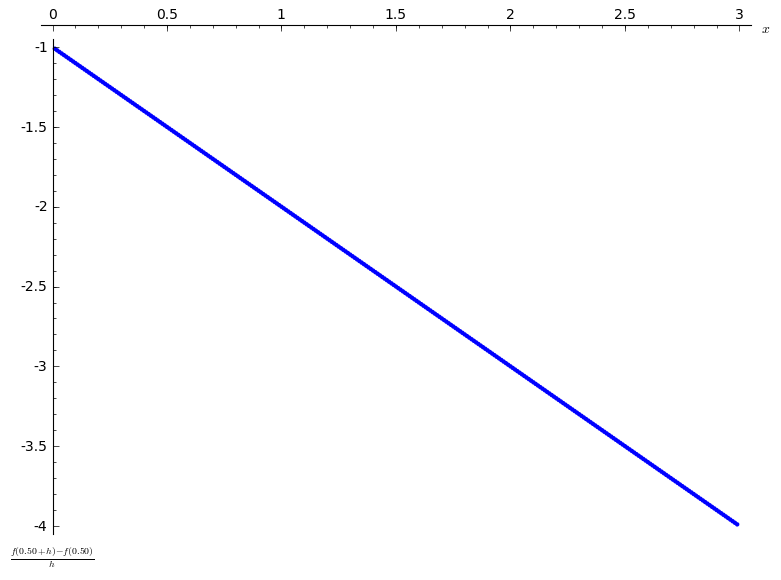
\includegraphics[width=8cm]{sage1.png}
\end{center}
\caption{The derivative of $f(x)=1-x^2$ at $x=.5$ converging to -1 as $h\to0$.}
\end{figure}

If we want to plot the tangent at a point $\alpha$ to a function we can use the following:

\begin{align}
y=&ax+b&&\text{(definition of a straight line)}\nonumber\\
  &f'(a)x+b&&\text{(definition of the derivative)}\nonumber\\
  &f'(a)x+f(a)-f'(a)a&&\text{(we know that the line intersects $f$ at $(a,f(a))$}\nonumber
\end{align}

We can combine this with the approach of the previous piece of code to see how the tangential line converges as the limiting definition of the derivative converges:

\begin{verbatim}
def convergetangentialline(f, a, x1, x2, nbrofplots=50, epsilon=.1):
    """
    Function to make a tangential line converge
    """
    clrs = rainbow(nbrofplots)
    k = 0
    h = epsilon
    p = plot(f, x, x1, x2)
    while k < nbrofplots:
        tangent(x) = fdash(f, a, h) * x + f(a) - fdash(f, a, h) * a
        p += plot(tangent(x), x, x1, x2, color=clrs[k])
        h += epsilon
        k += 1
    return p
\end{verbatim}

The plot shown in Figure \ref{lines} shows how the lines shown converge to the actual tangent to $1-x^2$ as $x=2$ (the red line is the `closest' curve).

\begin{figure}[!htbp]
\begin{center}
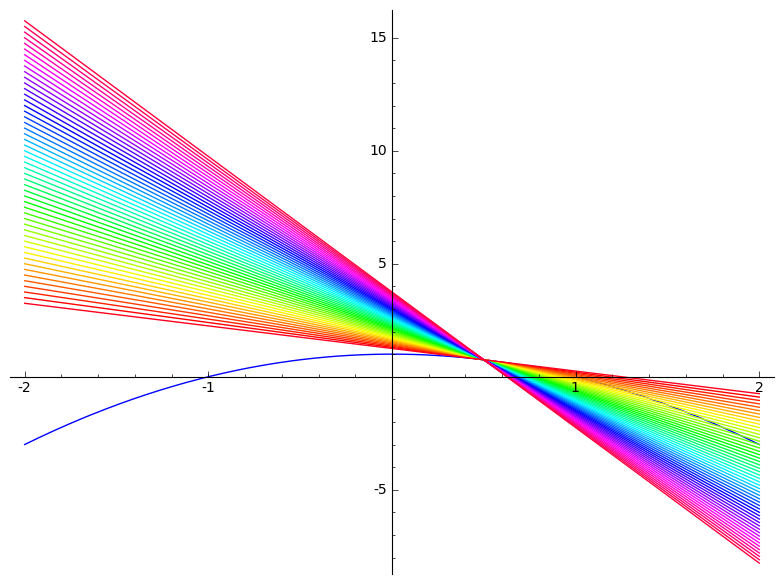
\includegraphics[width=8cm]{sage0.png}
\end{center}
\caption{Lines converging to the tangent curve as $h\to0$.}\label{lines}
\end{figure}

Note here that the last plot is given using the \textbf{real} definition of the derivative and not the approximation.

\section{Conclusions}

In this report I have explored the limiting definition of the limit showing how as $h\to 0$ we can visualise the derivative of a function. The code involved \url{https://sage.maths.cf.ac.uk/home/pub/18/} uses the differentiation capabilities of Sage but also the plotting abilities.

There are various other aspects that could be explored such as symbolic differentiation rules. For example:

$$\frac{dx^n}{dx}=(n+1)x^{n}\text{ if }x\ne-1$$

Furthermore it is interesting to not that there exists some functions that \textbf{are not} differentiable at a point such as the function $f(x)=\sin(1/x)$ which is not differentiable at $x=0$. A plot of this function is shown in Figure \ref{notdiff}.

\begin{figure}[!htbp]
\begin{center}
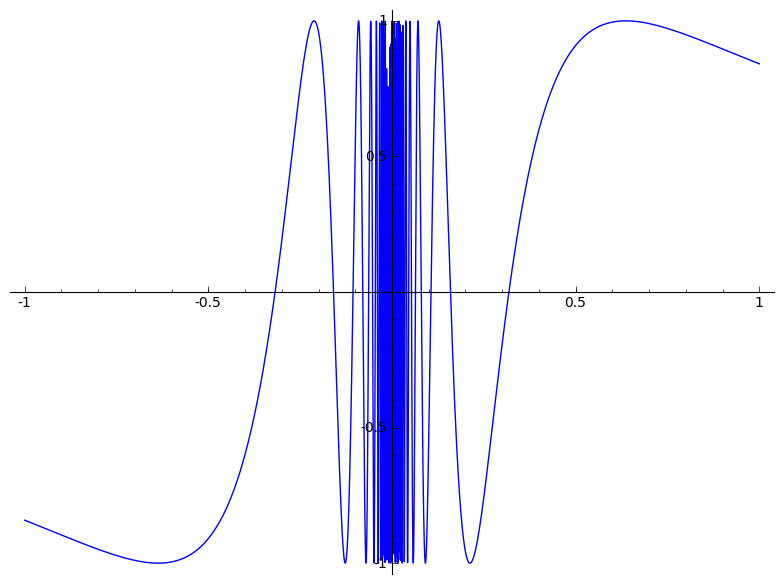
\includegraphics[width=8cm]{sage2.png}
\end{center}
\caption{None differentiable function at $x=0$.}\label{notdiff}
\end{figure}


\bibliographystyle{plain}
\bibliography{bibliography.bib}
\end{document}